\documentclass[11pt]{article}

\usepackage{microtype}
\usepackage{amsmath}
\usepackage{float}
\usepackage[colorlinks, urlcolor = blue]{hyperref}

\usepackage{graphicx}
\usepackage{caption}
\usepackage{subcaption}

\title{\textbf{Motion Estimation from optical flow}}
\author{ Moritz Loos 112385 }
\date{ Winter term 2014/15 }
\begin{document}
	
	\maketitle

	\section{Abstract}
	The goal of the project was to estimate the motion of a uav using a stereo camera system with help of the optical flow in the stereo images.

	\section{Introduction}
	The term optical flow describes the tracking of points from one image to another. Generally there are two possible approaches:
	At first we try to track every single pixel from frame to frame(called optical-field matching in the  following). In order to reduce the number of points to track we can use an interval to determine points to track (e.g. tracking every tenth pixel within every frame). The second approach would be tracking defined features instead of every pixel in every frame(feature-based matching).
	
	\begin{figure}[H]
	        \centering
	        %LINKS
	        \begin{subfigure}[b]{0.45\textwidth}
	                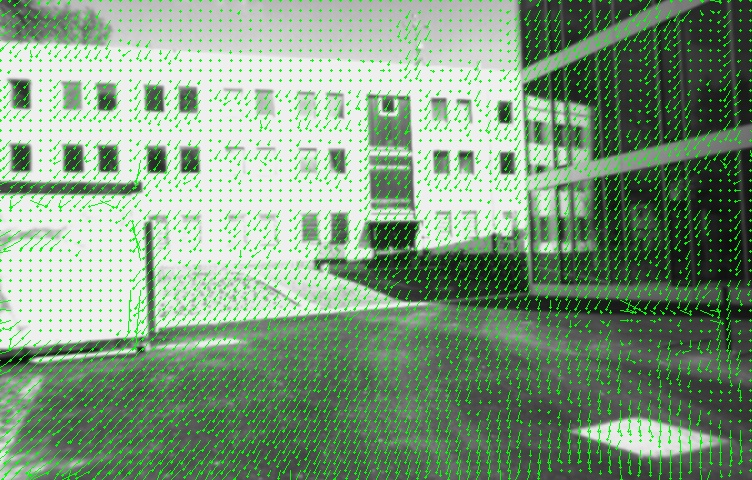
\includegraphics[width=0.45\textwidth]{images/farneback.jpg}
	                \caption{DESCRIPTION}
	                \label{fig:optical-field-matching}
	        \end{subfigure}\hfill 
	        %RECHTS
	        \begin{subfigure}[b]{0.45\textwidth}
	                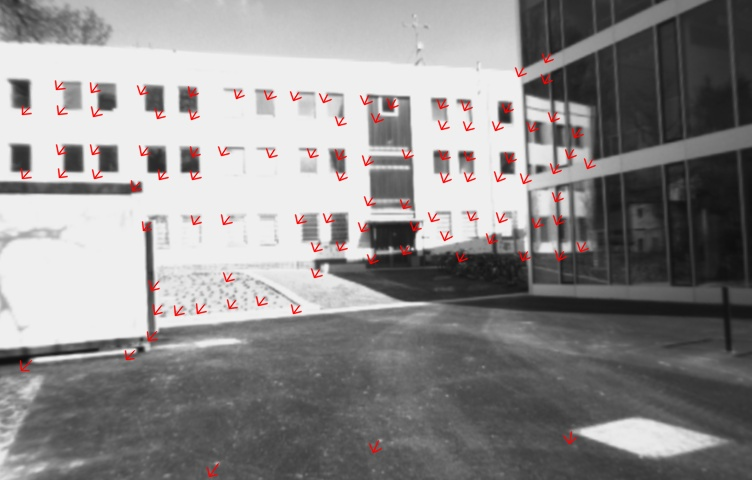
\includegraphics[width=0.45\textwidth]{images/feature-based-matching.jpg}
	                \caption{DESCRIPTION}
	                \label{fig:feature-based-matching}
	        \end{subfigure}
	\end{figure}
	
	Using optical-field matching the number of points is much higher than in feature-based matching. Also the distribution of points is much better. On the other side the number of outliers as well as the compuational effort are growing.
	[Obviously you have with the optical field approach much more points and especially a better distribution of points, but it is much more slower and has much more outliers.]

	In order to make the framework portable and stable (for the future use as a method for realtime flight-path detection) the basis is a feature-based matching algorithm.
	[i decided to use the feature-based matching because it is much more stable and faster than the other approach.]

	Unfortunately a simple mapping of optical flow vectors to the motion of a camera is just possible when some special constraints are fulfilled.
	\begin{enumerate}
	  \item The scene has to be static
	  \item The scene has to be parallel to the image plane of the camera
	  \item The scenes height has to be predefined.
	\end{enumerate}
	
	That means the camera has to look down permanently.
	[The scene have to be static and have to lie parallel to the image plane of the camera and in a defined height. That means the camera have to look permanent down.]

	\begin{figure}[H]
		\centering
		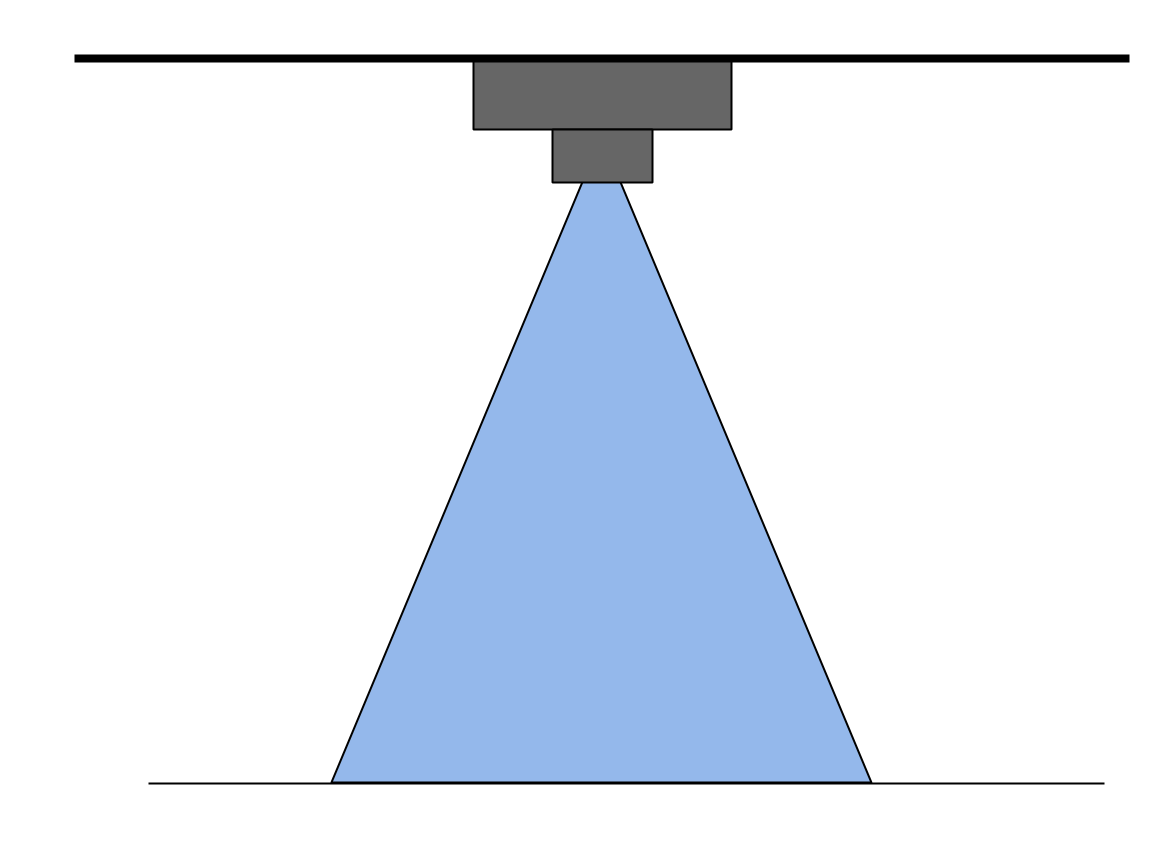
\includegraphics[width=\textwidth]{images/look_down.png}
		\caption{FOO}
		\label{fig:BAR}
	\end{figure}

	
	If all these constraints are fulfilled it is possible to estimate the motion of the camera using the length and the direction of the optical flow vectors.
	[If this constraints are given you could estimate the motion using the length and direction of the optical flow vectors.]

	\begin{figure}[H]
	        \centering
	        %LINKS
	        \begin{subfigure}[b]{0.45\textwidth}
	                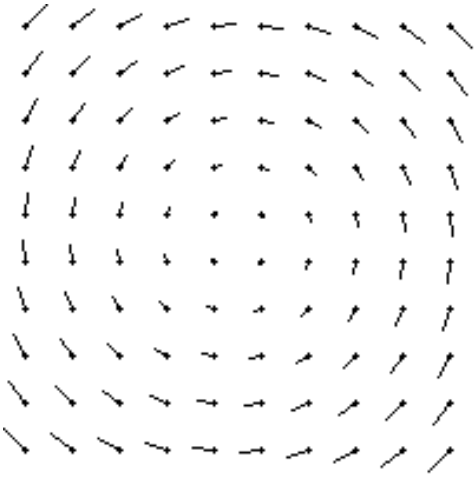
\includegraphics[width=0.45\textwidth]{images/rotation.png}
	                \caption{rotation}
	                \label{fig:FOO}
	        \end{subfigure}\hfill 
	        %RECHTS
	        \begin{subfigure}[b]{0.45\textwidth}
	                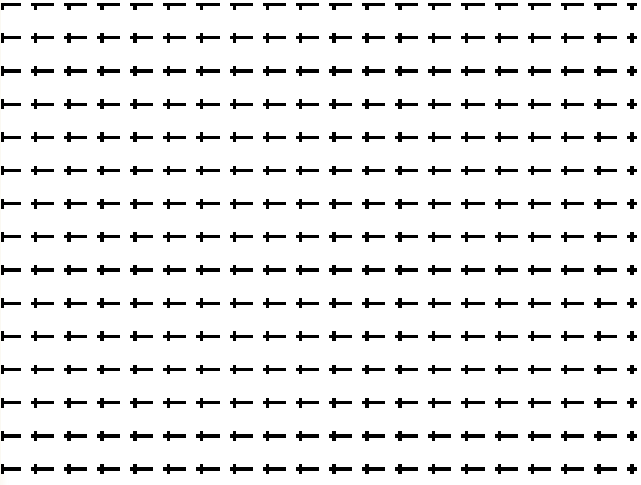
\includegraphics[width=0.45\textwidth]{images/translation.png}
	                \caption{translation}
	                \label{fig:FOO}
	        \end{subfigure}
	\caption{http://cvpr.uni-muenster.de/teaching/ss09/computerVisionSS09/script/CV08-Bewegungsanalyse.pdf}

	% Oder du nimmst ein \cite{FOO} und gibst das paper als eine der references an, das wuerde ich glaube ich so machen.
	\end{figure}

	As it is not possible for us to hold this constraints 
	Because we can’t hold this constraints we had to find other approaches.

	\section{Settings}
	The system we are using is a calibrated stereo rig [\cite{malik-hiller-2015}] and all values are defined like described in figure [figure [ref{fig:foo}]]. Where $P$ represents the projection matrix of the current camera($P_L$ is defined as the projection matrix from the left camera in frame 1 to the left camera in frame 2). $C$ describes the current camera image.
	%ich schreib dir den figure kram jetzt nicht nochmal hin, du weisst ja wie das geht.
	
	\begin{figure}[ht!]
		\centering
		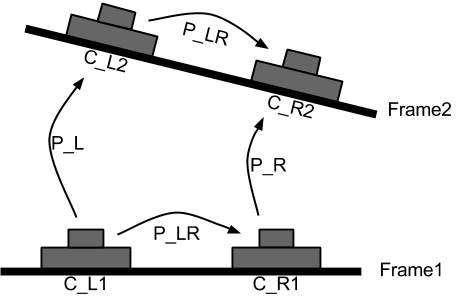
\includegraphics[width=90mm]{images/camera_setup.png}
		\caption{camera setup \label{overflow}}
	\end{figure}
	
	\section{visual odometry}
	In order to estimate the motion we need to find corresponding points in all 4 images. Our approach for performing visual odometry is represented in figure [] and is explained in the following.

	
	\begin{figure}[ht!]
		\centering
		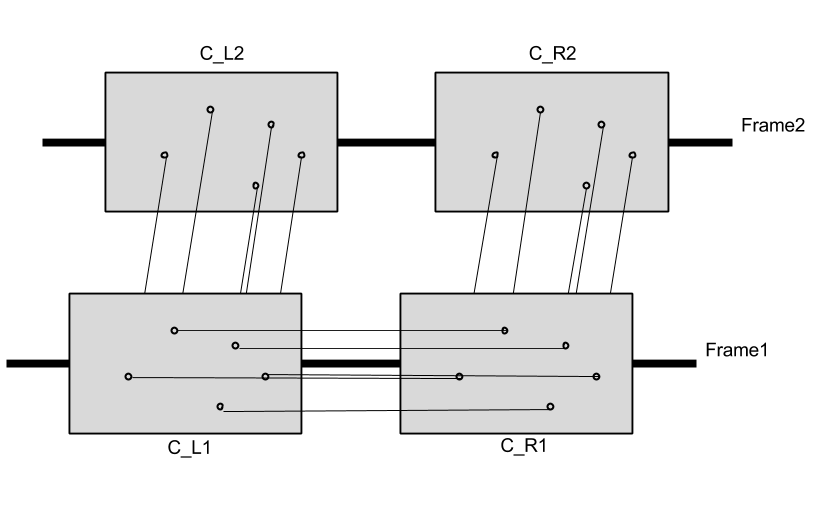
\includegraphics[width=90mm]{images/image_setup.png}
		\caption{image setup \label{overflow}}
	\end{figure}
	
	We start to detect features in $C_{L1}$ with the Shi-Tomasi Corner detector that is implemented in OpenCV. The Shi-Tomasi approach is a faster and more stable modification of Harris Corner detector [CITE]. 

	\begin{figure}[ht!]
		\centering
		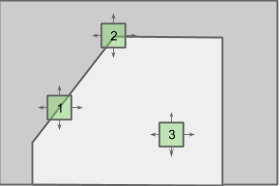
\includegraphics[width=90mm]{images/tomasi.png}
		\caption{Shi-Tomasi approach \label{overflow}}
	\end{figure}

	Features are characterized by their gradiation and the direction of the gradiation. With analyzing the eigenvalues of Window pattern arround a pixel is it possible to decide if the point is a corner, an edge or neither of them. In figure [] are shown different window pattern with different gradiation. The first pattern is an edge because there is no change of gradiation along the edge direction. Second pattern is a corner because there are changes in both directions. Last pattern has no change in any direction and is for this reason just classified as a flat surface (no feature). The Shi-Tomasi Corner detector is a really common approach, but an alternate could be the FAST feature detector or SURF (Speeded-Up Robust Features). 
	%(http://www.aishack.in/tutorials/the-shitomasi-corner-detector/, http://www.cs.ucf.edu/~mtappen/cap5415/lecs/lec5.pdf, http://www.informatikprojekt.de/uploads/dbv_report.pdf)

	After finding the features in $C_{L1}$ the algorithm tries to find the corresponding points in $C_{R1}$ and $C_{L2}$. Subsequently the points found in $C_{R1}$ are matched with the ones of $C_{R2}$
	To refind points in different images we use the lucas kanade algorithm [CITE] that is also part of the OpenCV library. 
	%[http://www.informatikprojekt.de/uploads/dbv_report.pdf]

	Beside SURF the Lukas Kanade Algorithm [CITE] is one of the most common methods to find features in an image. One requirement for this method is, that the intensity of a point in a specified window will not change from frame to frame. That is the main reason why the algorithm works best on systems with a high framerate, so that the movement between the single frames is very low.

			[The Lucas Kanade is beside SURF one of the most common algorithm to find features in an image. This method expects that the intensity of a point and the points in a specified window range don’t change from frame to frame. That's why this algorithm works well only for small motion (high fps). ]

	In this project we used the pyramidical approach of this algorithm. Therefor the reference image is downscaled to a certain numer of pyramidal layers [figure ()] with different resolutions. Afterwards the Lukas-Kanade Algorithm is called on each layer in ascending order (only in the range found previously). Using this method the algorithm is way faster, more robust and provides a better accuracy.
%[http://tu-dresden.de/die_tu_dresden/fakultaeten/fakultaet_forst_geo_und_hydrowissenschaften/fachrichtung_geowissenschaften/ipf/photogrammetrie/dateien/Westfeld2004.pdf]

			[In this project we used the pyramidical approach of this algorithm. Therefore the reference images is downscaled to a certain number of pyramidal layers showed in figure []. Than the lucas kanade tracking algorithm is called on each layer with a different resolution in ascending direction and only in the previously found range. With this approach the algorithm is faster, more robust and provides a better accuracy. 
%[http://tu-dresden.de/die_tu_dresden/fakultaeten/fakultaet_forst_geo_und_hydrowissenschaften/fachrichtung_geowissenschaften/ipf/photogrammetrie/dateien/Westfeld2004.pdf]]

	\begin{figure}[ht!]
		\centering
		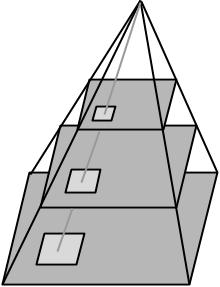
\includegraphics[width=90mm]{images/pyramidical.png}
		\caption{pyramedical approach of lucas kanade \label{overflow}}
	\end{figure}
	
	In order to prevent wron associations between points, outliers have to be deleted. Therefor OpenCV provides the findFundamentalMat() method using RANSAC. Although the method is doing what it is supposed to do, it finds too many good points (inliers) and declares them as outliers, and vice versa. Because it is quiet difficult to retrace the wrong definition of points we have to define inliers manually. One good approach therefor is the constraint of having a rectified stereo camera system. The flow vectors between $C_{L1}$ and $C_{R1}$ as well as $C_{L2}$ to $C_{R2}$ have to be horizontal on the images (epipolar geometry). If that is not the case we delete this point in all four frames. The following figure shows the inliers, represented as green arrows as well as the outliers represented as red arrows.
	
	\begin{figure}[ht!]
		\centering
		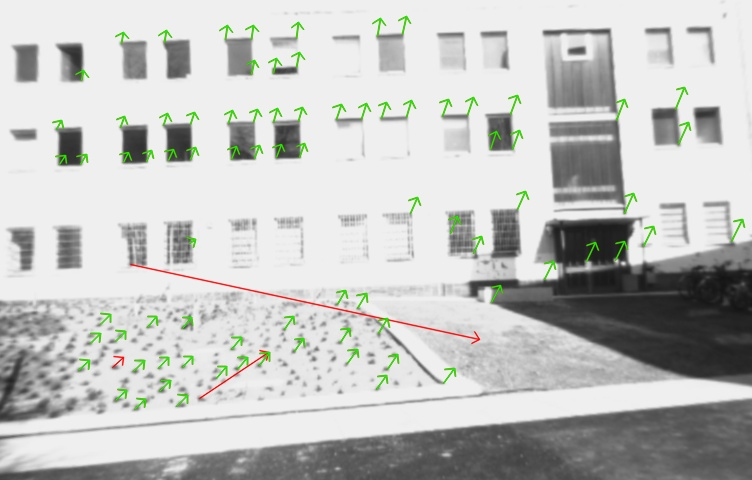
\includegraphics[width=90mm]{images/inlier_outlier3.jpg}
		\caption{inlier (green) and outlier (red) \label{overflow}}
	\end{figure}
	

	\section{Motion Estimation}
	
	Motion Estimation:
	Estimating motion between images is a hard task with many different approaches. Most of them use the projection matrix computed out of the essential matrix. The matrices we need are computed separately (left and right) between the current and the previous frame using detected features as correspondence points. Next we have to calculate the essential matrix as well as the camera matrices using the formula in figure [] [CITE: hartley and zisserman].
	\begin{align}
	  E = K’ \cdot F \cdot K
	\end{align}
	To obtain the perspective matrix we have to decompose the essential mat using svd [referenz auf irgendein paper]. Unfortunately the essential matrix can be decomposed to 4 different projection matrices and we have to find the right on. Therefore the points are triangulated using all four possible projection matrices with the goal to find the one where all points are in front of both cameras.
	[© Volker Rodehorst - Lecture Photogrammetric Computer Vision - WS 14/15]
	
	\begin{figure}[ht!]
		\centering
		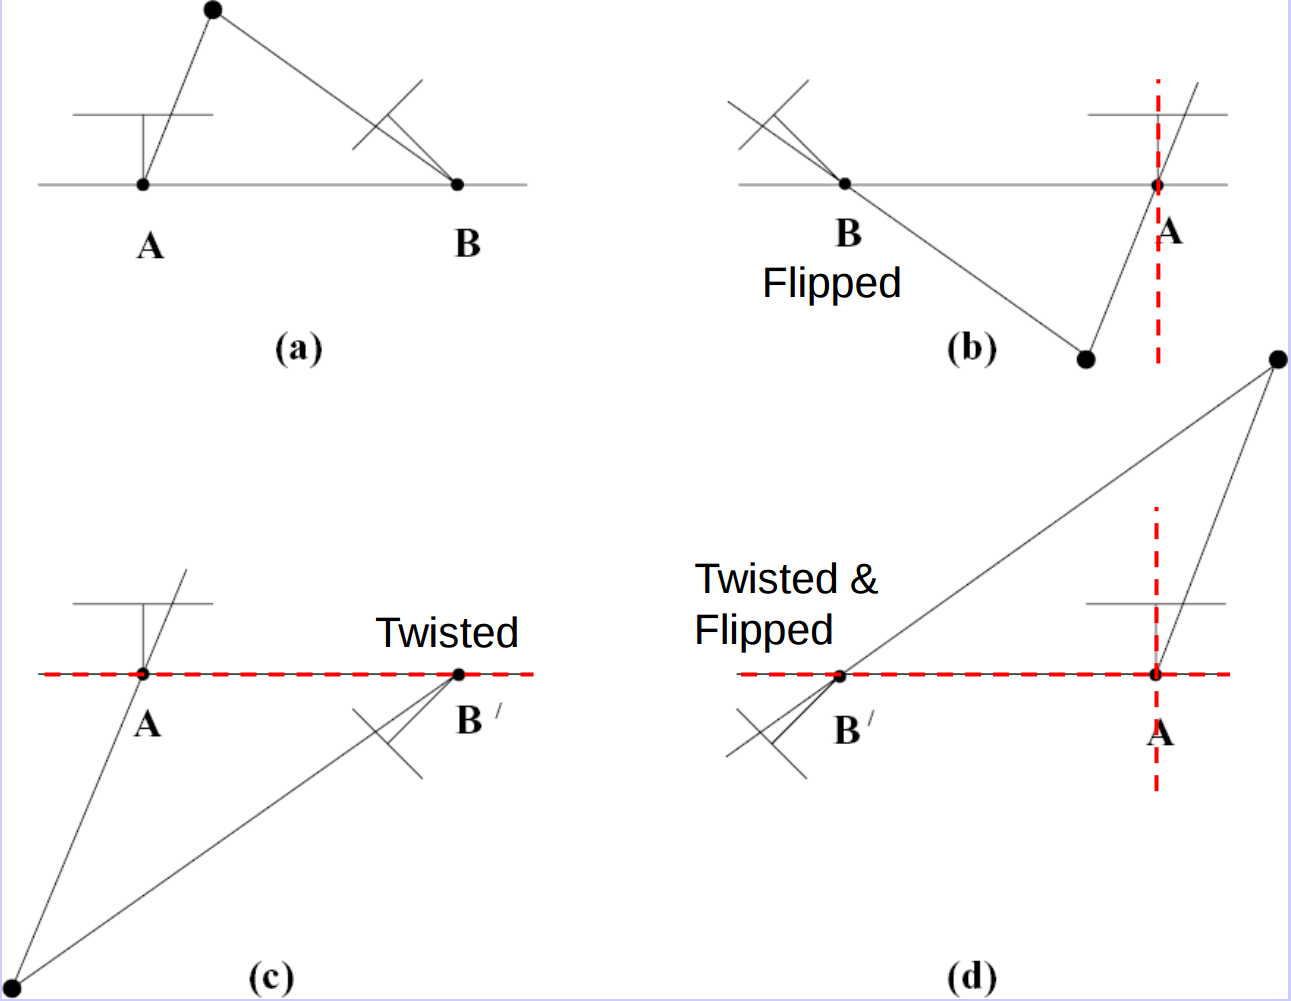
\includegraphics[width=90mm]{images/possible_P_Mats.png}
		\caption{inlier (green) and outlier (red) [© Volker Rodehorst - Lecture Photogrammetric Computer Vision - WS 14/15]
			 \label{overflow}}
	\end{figure}

	One problem left is that the found projection matrix is up to scale, which basically means that we just get the normalized direction vector (||T|| = 1) and the rotation of each camera. In order to get the correct scale factors we have to triangulate a reference pointcloud from the left to the right camera called $X$. This pointcloud is in the right scale because it is computed using $P_{LR}$ which already contains metric values. Next we triangulate points from the previous left image to the current left image resulting $X_L$, the same precedure is used to calculate $X_R$. To estimate te scale factor for $L$ and $R$ we just compare the poincoud with the reference $X$ as the folloginf formulas show: figure[] and figure[], [CITE paper knödelhorst].

	Improving the estimation can be done by just skipping frames where the motion estimation seems to fail and try to estimate the motion directly to the next valid frameset. To decide if the frameset is valid or not we can check against certain constraints. One of them is checking whether the determinant of $E$ is zero 
	%[http://en.wikipedia.org/wiki/Essential_matrix#Properties_of_the_essential_matrix]
	, the determinannt of a valid rotation matrix should be either positive or negative one. To determine a good fundamental matrix we need a minimum number of detected inliers. Also we have to define a maximum motion per frame as a maximum of one meter, because moving more than one meter with a framerate of either 30fps (binned) or 60fps is not realistic and can be declared as wrong. If one of this constraints cannot be fulfilled we skip the frameset and check the next one always remembering the last valid frameset. The method is robust as long we do not skip more than 4 frames because finding corresponding points after 4 frames is hard and if there is a circular motion nearly impossible. 

	\begin{figure}[ht!]
		\centering
		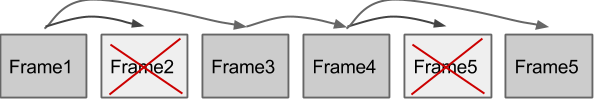
\includegraphics[width=90mm]{images/skipFrames.png}
		\caption{approach of skipping frames \label{overflow}}
	\end{figure}
	
	As described above there exist a lot of methods in the field of visual odometry. Beside the presented one we implemented two other approaches.
	The Perspective-n-point method is another way to estimate motion using a stereo-vision system. Therefor we have to find 3D-point to 2D-image-point correspondences. These are easy to gather using triangulation. Fortunately this method is included as RANSAC in OpenCV. The main idea is to use the dependency between 2D and corresponding 3D points. 2D points are here described as the multiplication of the projection matrix and the 3D-points as explained in the following formula [figure].
%	[http://homepages.inf.ed.ac.uk/rbf/CVonline/LOCAL_COPIES/MARBLE/high/pia/solving.htm]
	
	Second approach is to compare the orientation of the pointcloud triangulated in frame i to the point cloud triangulated in frame i+1 (see figure []).
	The whole method is explained in (cite paper hier einfuegen ([Combining Stereo Vision and Inertial Navigation System])).

	\begin{figure}[ht!]
		\centering
		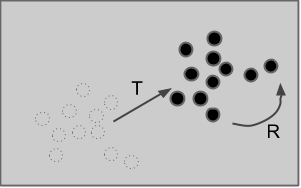
\includegraphics[width=90mm]{images/pointcloud_orientation.png}
		\caption{approach of pointclout orientation \label{overflow}}
	\end{figure}
	
	\section{Results}
	Using the first approach we gathered some useful results. We used the stereosystem connected to a notebook and walked around the Digital-Bauhaus-Lab in Weimar. Visually the estimated path matches to the one we walked. But as we take a deeper look on the results we can see that the start and end position is not matching though the test began and end in the exact same location. To express the added error in numbers we can take a look at the coordinates estimated. We started at [0, 0, 0] and stopped at [-0,23m, -5.46m, -1.9m], which means we drifted by $\pm$ 6m in every direction. At this point we were not able to gather any useful results using the other tow approaches.

	\section{Issues}

	There are many different factors for good results when trying to estimate the motion out of stereo camera images. Obviously the corresponting points and their accuracy are the most important factor. The quality as well as the distribution of points are two very important components, but also the number of correct points. For a good triangulation it is essential that the found features are not too far awar e.g at the horizon. The reason for that is the small distance between the points, so it is really hard to differ which feature belongs to another within different frames and camera images. Whereby the same problem occurs with too small translation. Another issue which can lead to problems is the size of the baseline between the cameras. If it is too small the triangulation might fail because of very low angles, if it is too big the number corresponding points can be to less.
	
	
	\section{Future work}
	In order to make the algorithm more robust it is important that the error from frame to frame does not grow more. Bundle adjustment could be a useful approach to solve this problem. A comparison between these three methods would be useful to evaluate the best method for a specific setup. Another idea would be to combine the methods to get a system which is able to cope with very different situations. The current code is basically written to be used in a comfortable way, therefor an implementation with focus on performance and stability would be important. Live test should be also done in order to evaluate the current performance and robustness.

\end{document}